%% It is just an empty TeX file.
%% Write your code here.

\section{Implementation}
\label{sec:implementation}
% logo definitions
\newcommand{\logoFleur}{%
  \begingroup\normalfont
  \includegraphics[height=1.2\fontcharht\font`\B]{img/logo/fleur.png}%
  \endgroup
}
\newcommand{\logoAiida}{%
  \begingroup\normalfont
  \includegraphics[height=1.0\fontcharht\font`\B]{img/logo/aiida.png}%
  \endgroup
}
\newcommand{\logoAiidalab}{%
  \begingroup\normalfont
  \includegraphics[height=1.0\fontcharht\font`\B]{img/logo/aiidalab.png}%
  \endgroup
}
\newcommand{\logoBinder}{%
  \begingroup\normalfont
  \includegraphics[height=1.2\fontcharht\font`\B]{img/logo/binder.png}%
  \endgroup
}
\newcommand{\logoBokeh}{%
  \begingroup\normalfont
  \includegraphics[height=1.2\fontcharht\font`\B]{img/logo/bokeh.png}%
  \endgroup
}
\newcommand{\logoDash}{%
  \begingroup\normalfont
  \includegraphics[height=1.2\fontcharht\font`\B]{img/logo/dash.png}%
  \endgroup
}
\newcommand{\logoDocker}{%
  \begingroup\normalfont
  \includegraphics[height=1.2\fontcharht\font`\B]{img/logo/docker.png}%
  \endgroup
}
\newcommand{\logoHoloviews}{%
  \begingroup\normalfont
  \includegraphics[height=1.2\fontcharht\font`\B]{img/logo/holoviews.png}%
  \endgroup
}
\newcommand{\logoHvplot}{%
  \begingroup\normalfont
  \includegraphics[height=1.2\fontcharht\font`\B]{img/logo/hvplot.png}%
  \endgroup
}
\newcommand{\logoJavascript}{%
  \begingroup\normalfont
  \includegraphics[height=1.2\fontcharht\font`\B]{img/logo/javascript.png}%
  \endgroup
}
\newcommand{\logoJupyter}{%
  \begingroup\normalfont
  \includegraphics[height=1.2\fontcharht\font`\B]{img/logo/jupyter.png}%
  \endgroup
}
\newcommand{\logoMatplotlib}{%
  \begingroup\normalfont
  \includegraphics[height=1.2\fontcharht\font`\B]{img/logo/matplotlib.png}%
  \endgroup
}
% \newcommand{\logoMpld3}{%
%   \begingroup\normalfont
%   \includegraphics[height=1.2\fontcharht\font`\B]{img/logo/mpld3.png}%
%   \endgroup
% }
\newcommand{\logoPanel}{%
  \begingroup\normalfont
  \includegraphics[height=1.2\fontcharht\font`\B]{img/logo/panel.png}%
  \endgroup
}
\newcommand{\logoParam}{%
  \begingroup\normalfont
  \includegraphics[height=1.2\fontcharht\font`\B]{img/logo/param.png}%
  \endgroup
}
\newcommand{\logoPlotly}{%
  \begingroup\normalfont
  \includegraphics[height=1.2\fontcharht\font`\B]{img/logo/plotly.png}%
  \endgroup
}
\newcommand{\logoPython}{%
  \begingroup\normalfont
  \includegraphics[height=1.2\fontcharht\font`\B]{img/logo/python.png}%
  \endgroup
}
\newcommand{\logoPyviz}{%
  \begingroup\normalfont
  \includegraphics[height=1.2\fontcharht\font`\B]{img/logo/pyviz.png}%
  \endgroup
}
\newcommand{\logoSeaborn}{%
  \begingroup\normalfont
  \includegraphics[height=1.2\fontcharht\font`\B]{img/logo/seaborn.png}%
  \endgroup
}

%%% Local Variables:
%%% mode: latex
%%% TeX-master: t
%%% End:


\newcommand{\theimage}{\includegraphics[width=0.8\linewidth]{img/module_design.png}}% Shorthand
\begin{frame}\frametitle{Module Design Goals}
    \begin{columns}
        \begin{column}{.4\textwidth}
            \centerline{\theimage}
        \end{column}
        \begin{column}{.6\textwidth}
            \visible<1->{Multifunctionality:
            \begin{itemize}            
            \item automated workflows like in \logoAiida{}
            \item manual data analysis with Python
            \end{itemize}}
            \visible<2->{\hdashrule{\textwidth}{1pt}{1pt}
            \begin{itemize}
            \item no boilerplate code!
            % \vspace{0.5em}
            \end{itemize}}
            \visible<3->{\hdashrule{\textwidth}{1pt}{1pt}
            \begin{itemize}
            \item Desktop \faDesktop{}
            \item Web \faServer{} \faArrowRight{} \faGlobe{} like in \logoAiidalab{}
            \end{itemize}}
        \end{column}
    \end{columns}
\end{frame}
% Talking Notes:
% TODO

\subsection{Preprocessor}
\label{sec:preprocessor}

\renewcommand{\theimage}{\includegraphics[width=1.2\linewidth]{img/reader_flowchart4.png}}% Shorthand
\begin{frame}\frametitle{Preprocessor Module}
    \begin{columns}
        \begin{column}{.55\textwidth}
            \visible<3->{\centerline{\theimage}}            
        \end{column}

        \begin{column}{.4\textwidth}
            \visible<1->{Input: Fleur calculation results stored in Hierarchical Data Format
            (HDF).}
            \visible<2->{Combining \emph{Python AB\(C^1\) and \emph{type
                  introspection}} enables concise \textbf{Recipes} for different applications:}
            \begin{itemize}
            \item<4-> \faArrowRight{} attribute dependency resolution
            \item<5-> \faArrowRight{} modular output types
            \end{itemize}
        \visible<2->{\textsuperscript{1}Abstract Base Class}            
        \end{column}
    \end{columns}
\end{frame}
% Talking Notes:
% - HDF: like a file system with metadata annotation
% - Recipe: build class at runtime (introspection), with transformed attributes (HDF datasets) and
%   application-specific functions, and instantiate object.
% - Dependency resolution: user does not have to take care of order in which
%   arguments are processed (alphabetic ordering)
% - Transforms Dependency example: coordinate transformation
% - Reusability: new recipes may be composed for different workflows with minimal effort
% - Abstract base classes define general and specific Transforms and Output Types
% - Output type example: FleurBands

\begin{frame}\frametitle{Data Selection for Visualization}    
    Application Band Structure Viz.: from 4D discrete weighted points to 2D bands.
    \begin{align*}
      W^{\text{eff}}_{s,k,\nu} = \left( \frac{\sum\limits_{\substack{g \in \text{groups} \\ l \in \text{characters}}} n_{s,k,\nu,g,l} N_g}{\sum\limits_{\substack{g \in \text{all groups} \\ l \in \text{all characters}}} n_{s,k,\nu,g,l} N_g} \right) \left(W_{s,k,\nu}^{\text{unf}}\right)^\alpha
    \end{align*}
    \vspace{1em}
    \begin{itemize}
    \item<2-> \(W^{\text{eff}}_{s,k,\nu}\): effective weight
    \item<3-> \(s\) spin, \(k\) point on \(k\)-path, \(\nu\) band, \(g\)
        group, \(l\) character
    \item<4-> \(n_{s,k,\nu,g,l}\): State-specific \(l\)-like charge
    \item<5-> \(N_g\): no. of atoms in group         
    \item<6-> \(W_{s,k,\nu}^{\text{unf}}\): unfolding weight; \(\alpha =0\implies \) no unfolding
    \end{itemize}

    
\end{frame}
% Slide notes:
% - Reference: Bluegel FLAPW https://www.fz-juelich.de/SharedDocs/Downloads/PGI/PGI-1/DE/SB_NIC_pdf.pdf?__blob=publicationFile
% - indices: nu = band index, mu = muffin tin (i.e. atom, probably corresponds
% to atom group index), l = angular
% quantum number?
% - s = spin, k = k vector, g atom group, G_g atoms_per_group
% - alpha = unfolding weight exponent
% 
% Talking Notes:
% - get_data method

\begin{frame}
    \frametitle{Data Selection for Viz}
    % ballpark calculation: spins 2, k 500, bands 400, groups 20, chars 4
    Typically, \(\sim 10^7\) data points are accessed.
    \pause
    \vspace{2em}
     
    Optimizations:
    \pause
    \begin{itemize}
    \item reshaping \((k,\nu) \rightarrow (k \cdot \nu)\)
        \pause
    \item weight filter \(t\): \(W^{\text{eff}}_{s,k,\nu} > t\)
        \pause
    \item using optimized \texttt{numpy} functions for tensor product
        \pause
    \item buffering on selection change
    \end{itemize}
    \pause 
    \faArrowRight{} Speedup \(\sim 10^2\)
\end{frame}

\subsection{Interactive Visualization}
\label{sec:visualization}

\renewcommand{\theimage}{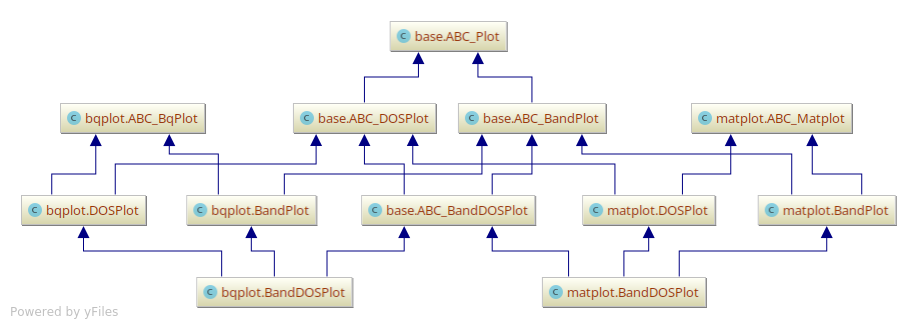
\includegraphics[width=1.1\linewidth]{img/pycharm_uml/matplot.png}}% Shorthand
\begin{frame}\frametitle{Visualization Module}
    \begin{itemize}
    \item<1-> Combine \emph{Python ABC} and \emph{multiple inheritance}
    \item<2-> \faArrowRight{} maximizes code reuse for different applications
        and viz. libraries employed
    \end{itemize}    
    \visible<3->{\centerline{\theimage}}
\end{frame}

\subsection{Desktop Frontend}
\label{sec:desktop-frontend}

\begin{frame}\frametitle{Desktop Frontend}
    Choice of GUI Toolkit: \textbf{TKinter} over (Kivy, PySide/PyQt, ...)

    Choice of Plotting tool: \textbf{matplotlib}
\end{frame}

\subsection{Web Frontend}
\label{sec:web-frontend}

\renewcommand{\theimage}{\includegraphics[width=1.0\linewidth]{img/py-viz-landscape.png}}% Shorthand
\begin{frame}\frametitle{Web Frontend}
    \visible<1->{The Python Visualization Landscape as of 2017...}
    \visible<2->{
      \centerline{\theimage}
      \begin{tiny}
          \href{https://github.com/rougier/python-visualization-landscape}{Python
            Visualization Landscape} by \href{https://github.com/rougier}{rougier} / BSD-2    
      \end{tiny}} 
\end{frame}

\begin{frame}\frametitle{Web Frontend}
    \begin{itemize}
    \item<1->Needed: a \textbf{survey} of OSS Frameworks for building a Web
        Dashboard using \textbf{only} \logoPython{}.
    \item<2-> Selection Process: \emph{Framework supports...}
        \begin{itemize}
        \item<3-> I. \emph{... interactive graphical control
              elements ('widgets') to control plots}
        \item<4-> II. \emph{... easy deployment}
        \item<5-> III. \emph{... some actual plotting libraries}
        \end{itemize}        
    \end{itemize}
\end{frame}

\begin{frame}\frametitle{Web Frontend}
    \begin{table}
        \resizebox{\textwidth}{!}{%
          \begin{tabular}{c||c|c|c|c}
            \visible<1->{I. \textbf{Widgets} & \logoJupyter{} jupyter & pyviz \logoPanel{} panel & \logoBokeh{} bokeh & \logoDash{} dash \\\hline
            Languages & \logoPython{} & \logoPython{} & \logoPython{} / \logoJavascript{} & \logoPython{} / \logoJavascript{} \\\hline}
            \visible<2->{II. \textbf{Deployment} & & & & \\
            - Jupyter & \faCheck{} & \faCheck{} & \faCheck{} & \faCheck{} \\
            - Standalone\footnote{Excluded: writing from scratch using Flask} & (\logoBinder{}, \logoDocker{})\footnote{workaround. See also: \href{https://github.com/oschuett/appmode}{appmode}, \href{https://github.com/QuantStack/voila}{voila}, \href{https://github.com/minrk/thebelab}{thebelab}} & \logoBokeh{} server & \logoBokeh{} server & \logoPlotly{} plotly \\\hline}
            \visible<3->{III. \textbf{Plots}\footnote{interactive only}  & & & & \\
            - 2D & \logoMatplotlib{} mpl, bqplot, \textbf{all}  \faArrowLeft{} & \logoHvplot{} hvplot,  \faArrowRight{} \textbf{most} \faArrowLeft{}  & \logoBokeh{} & \logoPlotly{}\\
            - 3D & ipyvolume, \textbf{all}  \faArrowLeft{} & \faClose{} & \logoBokeh{} & \logoPlotly{}}
          \end{tabular}
        }
    \end{table}
\end{frame}
% Talking Notes:
% - Our decision:
%   - PyViz best (abstract GUI declaration supports Tkinter) but no 3D for atom plots, so out again
%   - Jupyter > (Bokeh, Dash) but expect deployment in AiiDAlab (JupyterHub) so simpler
%   - problem: standalone will now be harder, but maybe possible through binder
%   - 2D: matplotlib first cause same as Tkinter, for now
%   
 







% 

